\section{Search Suggestion}
We want the users to be able to enter the ingredients they have in their home, however it can be quite tedious to type in the full ingredient names of all the ingredients, so we want to aid the users by providing them with search suggestions as they type in the names. The user can press these search suggestions to quickly add the ingredient to the list of ingredients that the user has. 
We have decided that only the ingredients that are used in recipes can be added to list of ingredients that the user has. This means that the user is only able to enter ingredients that is already used by a recipe. The reason for this was that we did not want the user to be able to search for random text strings, or to get an empty search because none of their ingredients matched those in the recipes. 

When the users opens the application, all the ingredients are loaded into a list, this list of ingredients is then used for the search suggestions. Each time the user types in a letter, the input string is run through a regular expression trying to match the input string to an ingredient name in the list, the matching ingredients is added to a list and shown on the screen as a search suggestion. This can be seen in \autoref{lst:search}.
\pagebreak

\begin{lstlisting}[language=java, label=lst:search, caption={Search suggestions.}]
Pattern p = Pattern.compile("(^|\\s)" + query);

for (Ingredient ingredient : allIngredients) {
    Matcher matcher = p.matcher(ingredient.getSingular().toLowerCase());

    if (matcher.find()) {
        suggestionName.add(ingredient.getSingular());
    }
}
\end{lstlisting}

\begin{description}
\item[Line 1] \inline{Pattern.Compile()} returns a compiled form of the regular expression. The expression matches the start of a string or a space and then the input itself. 
\item[Line 3-4] We loop through the list of ingredients to see if the regular expression matches any of the ingredient names.
\item[Line 6-7] Each, if any, suggestion that is found is added to the suggestion list.
\end{description}

\begin{figure}[H]
\begin{minipage}[b]{0.5\columnwidth}
\centering
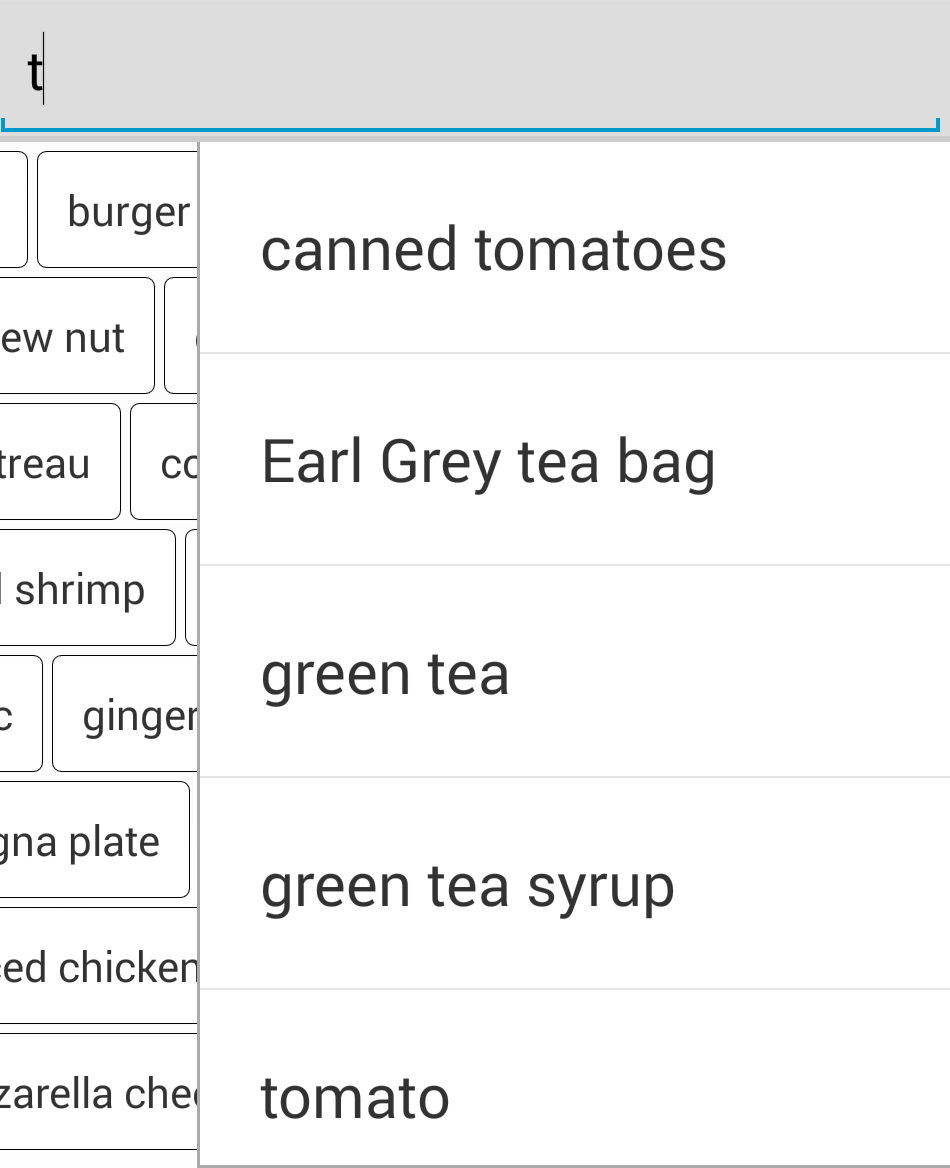
\includegraphics[width=0.7\columnwidth]{img/screenshots/searchSuggestion1.png}
\caption{Suggestions with a ``t''\label{fig:suggestt}.}
\end{minipage}
\hspace{0.5cm}
\begin{minipage}[b]{0.5\columnwidth}
\centering
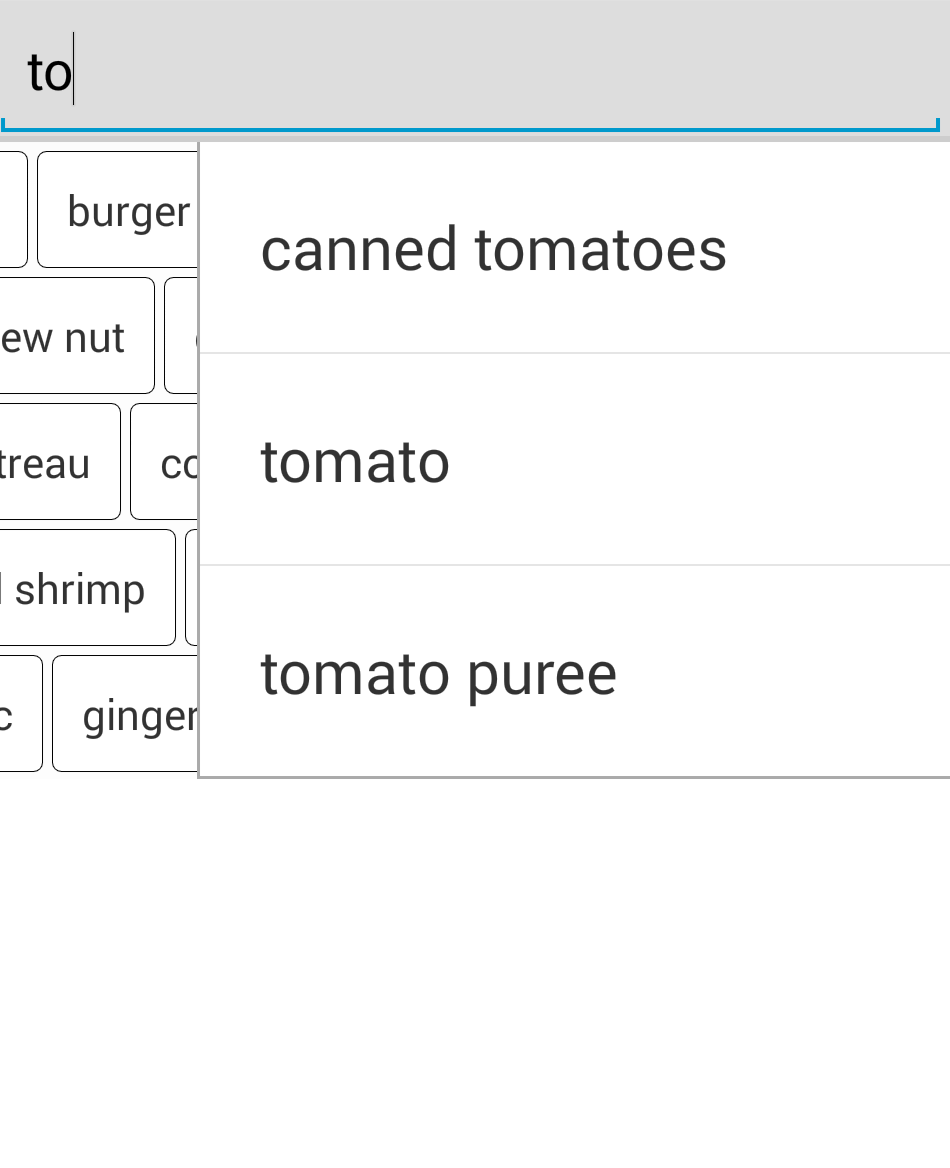
\includegraphics[width=0.7\columnwidth]{img/screenshots/searchSuggestion2.png}
\caption{Suggestions with ``to''\label{fig:suggestto}.}
\end{minipage}
\end{figure}

\autoref{fig:suggestt} and \autoref{fig:suggestto} shows two examples of how this works. When the user types in a ``t'' they get all ingredients where a part of the string starts with a ``t'', if the users continues and types an ``o'', the suggestions are updated and now only show the words where parts of the string starts with ``to''. 

The user can add ingredients to the word cloud in two ways, they can either type parts of the name as shown in \autoref{fig:suggestt} and \autoref{fig:suggestto} and press the correct suggestion in the list of suggestions or they can type parts, or the full name, and press the enter button on the keyboard. Doing this will add the first ingredient in the suggestion list to the search.